%%%%%%%%%%%%%%%%%%%%%%%%%%%%%%%%%%%%%%%%%%%%%%%%%%%%%%%%%%%%%
%% HEADER
%%%%%%%%%%%%%%%%%%%%%%%%%%%%%%%%%%%%%%%%%%%%%%%%%%%%%%%%%%%%%
\documentclass[a4paper,twoside,11pt]{article}

%% Language %%%%%%%%%%%%%%%%%%%%%%%%%%%%%%%%%%%%%%%%%%%%%%%%%
\usepackage[T1]{fontenc}

%\usepackage[ansinew]{inputenc}
\usepackage[utf8]{inputenc}	%supports Umlaute
%\usepackage{german, ngerman}
\usepackage{color}

\usepackage{lmodern} %Type1-font for non-english texts and characters

%% Packages for Graphics & Figures %%%%%%%%%%%%%%%%%%%%%%%%%%
\usepackage{graphicx} %%For loading graphic files
\usepackage{multicol}

%% Math Packages %%%%%%%%%%%%%%%%%%%%%%%%%%%%%%%%%%%%%%%%%%%%
\usepackage{amsmath}
\usepackage{amsthm}
\usepackage{amsfonts}
\usepackage{amssymb}

%% Line Spacing %%%%%%%%%%%%%%%%%%%%%%%%%%%%%%%%%%%%%%%%%%%%%
\usepackage[parfill]{parskip}    % Activate to begin paragraphs with an empty line rather than an indent

%% Other Packages %%%%%%%%%%%%%%%%%%%%%%%%%%%%%%%%%%%%%%%%%%%
\usepackage{a4wide} %%Smaller margins = more text per page.
\usepackage{fancyhdr} %%Fancy headings

%%%%%%%%%%%%%%%%%%%%%%%%%%%%%%%%%%%%%%%%%%%%%%%%%%%%%%%%%%%%%
%% DOCUMENT
%%%%%%%%%%%%%%%%%%%%%%%%%%%%%%%%%%%%%%%%%%%%%%%%%%%%%%%%%%%%%
\begin{document}

\pagestyle{fancyplain}

%% Title Page %%%%%%%%%%%%%%%%%%%%%%%%%%%%%%%%%%%%%%%%%%%%%%%
\title{Parallel Programming Assignment \#2} 
\author{Marcel Karsten -- 343619,\\ Patrick Lorenz -- 341922,\\ Richard Klemm -- 343635 }
\date{Due: Thursday, 24th May 2012} %%If commented, the current date is used.
\maketitle

%% Header on top of every page (yes, also on the title page!)
\rhead{Parallel Programming - TU Berlin, SS/12}
\lhead{}
\renewcommand{\headrulewidth}{0px}


%%%%%%%%%%%%%%%%%%%%%%%%%%%%%%%%%%%%%%%%%%%%%%%%%%%%%%%%%%%%%

\section{Exercise 1 - Sequential Overspecification}
Input of the algorithm are two strings (a, b) and a minimum matching length (K). The algorithm compares sequence \textit{a} to sequence \textit{b} and provides all matching substrings with at least K characters.

The first part of the algorithm (first nested for loops) fills the cells of the matrix L. Important are the diagonals that represent a specific starting points in the sequences. Every cell (i, j) of the matrix now indicates if the characters a[i] and b[j] match and how long the matching substring towards that point is. The diagonal on the bottom left (see example matrix) with values from 1 to 4 shows the matching substring "`Welt"` that is part of both sequences. The same stands for the diagonal on the top right (see example matrix) going from 1 to 5 with the substring "`Hallo"'.

The second part now selects the matching substrings that have at least K characters and prints the indices of the sequences and the matching length.


The example inputs a="'HalloWelt"' and b="'WeltHallo"' yield the following matrix 

$$L=
\begin{pmatrix}
	0 & 0 & 0 & 0 & 1 & 0 & 0 & 0 & 0 \\
	0 & 0 & 0 & 0 & 0 & 2 & 0 & 0 & 0 \\
	0 & 0 & 1 & 0 & 0 & 0 & 3 & 1 & 0 \\
	0 & 0 & 1 & 0 & 0 & 0 & 1 & 4 & 0 \\
	0 & 0 & 0 & 0 & 0 & 0 & 0 & 0 & 5 \\
	1 & 0 & 0 & 0 & 0 & 0 & 0 & 0 & 0 \\
	0 & 2 & 0 & 0 & 0 & 0 & 0 & 0 & 0 \\
	0 & 0 & 3 & 0 & 0 & 0 & 1 & 1 & 0 \\
	0 & 0 & 0 & 4 & 0 & 0 & 0 & 0 & 0
\end{pmatrix}
$$

\newpage
\section{Exercise 2 - Parallel Algorithm Design}
\textbf{(a) Foster's design methodology}

Foster's Methodology consist of four steps. Following the characteristics of our OpenMP algorithm concerning these steps are described.

Foster's Methodology:
\begin{enumerate}
	\item Partitioning
	\item Communication
	\item Agglomeration
	\item Mapping
\end{enumerate}

\textsc{1. Partitioning}

To partition the given problem the diagonals of the matrix can be used. The computations on these are independet of each other. So it is possible to assign one diagonal to one task. 

This leads to the advantage that the number of tasks grows with the problem size because with growing sequences the number of diagonals grows. Furthermore there are no redundant computations and the memory consumption is more efficient because only those matching substrings are saved that satisfy the value of the given K.

Disadvantages are that the different tasks do not have the same size and many tasks have to hold the same parts of the sequences in their memory.



\textsc{2. Communication}

As stated in the section before computations on the diagonals are independent of each other. Therefore there is no communication needed between the task. At the end of computations the results of the tasks have to be collected.

\textsc{3. Agglomeration}

It is possible to agglomerate tasks into one task by combining several diagonals. To increase locality the combined diagonals should be adjacent.

\textsc{4. Mapping}

The mapping of the tasks to processors/threads is done by the operating system or by the OpenMP library.

\textbf{(b) OpenMP}
Due to it's structure, the OpenMPAlgorithms are able to handle the large datasets to some extend, too. The amount of memory required is directly related to K, thus if K is large enough, the program does not run out space.

See source of classes OpenMPAlgorithm and OpenMPAlgorithmTasks.

\textbf{(c) Optimization}

Two concepts of optimization were deployed: Optimizations done automatically when configuring the compiler correctly and manually optimizing the code. The former was deployed in the  SequentialOptimizedAlgorithm and the CMakeLists.txt file; the latter in the SequentialOptimizedAlgorithm2 file.

As compiler optimization settings, the \textit{-O3}flag as well as the \textit{-march=native} flag were set.

\section{Exercise 3 - Benchmarking}

\begin{figure}[hbtp]
\caption{Single Speed Comparison}
\centering
\label{fig:seq_comp}
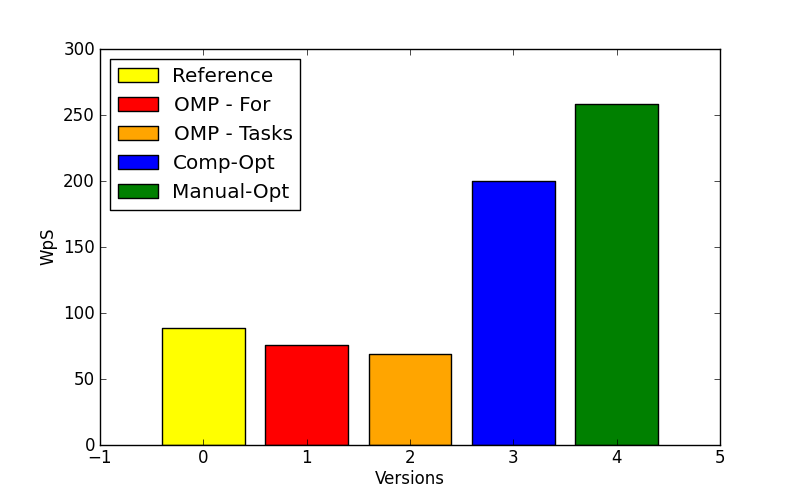
\includegraphics[scale=0.8]{seq.png}
\end{figure}

As a result of task two four different versions of the implementation were created. 
Figure[\ref{fig:seq_comp}] shows the average speed of three testruns of every version of the algorithm. The test was conducted using just one thread and matching length of one character. Thus, it shows the pure sequential speed.
The \textit{Reference} - Version is the originally given  algorithm with no optimizations applied, while \textit{Comp-Opt} is the same source with compiler optimizations enabled. \textit{Manual-Opt} is the manually optimized source code, with compiler optimizations still enabled.
\textit{OMP - For } is an OMP Version using a \textit{parallel for} construct and \textit{OMP - Tasks} uses the \textit{tasks} constructs.
Both OpenMP versions are slightly slower than the reference. That is maybe caused by additional overhead needed for thread initialization and  organization.

Both optimized sequential algorithms show a much better performance. Also, it can easily be seen that manual optimization using \textit{loop peeling} and \textit{loop unwinding} is well worth the effort if pure speed is needed. It still beats the compiler's optimizations and is almost three times faster than the reference implementation.

\begin{figure}[hbtp]
\caption{OpenMP Parallel For Loop}
\centering
\label{fig:omp_parallel}
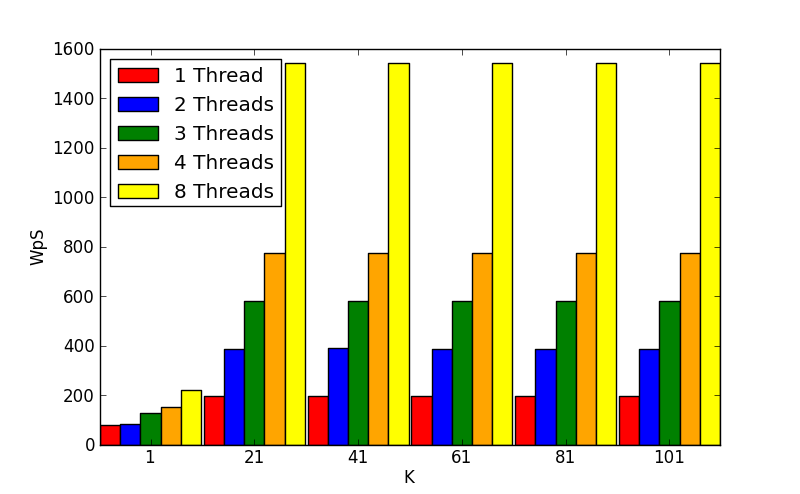
\includegraphics[scale=0.8]{omp_for.png}
\end{figure}

\begin{figure}[hbtp]
\caption{OpenMP Tasks}
\centering
\label{fig:omp_tasks}
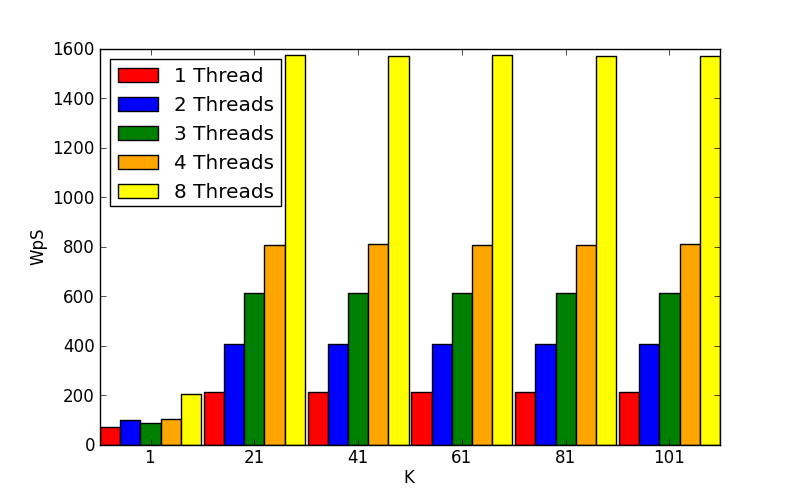
\includegraphics[scale=0.8]{omp_tasks.png}
\end{figure}

Figure[\ref{fig:omp_parallel}] and figure[\ref{fig:omp_tasks}] show a comparison of the two OpenMP versions described above using a  varying number of threads as well as varying matching lengths(\textit{K}). With $K=1$ the performance of the eight thread version is roughly the same as the manually optimized sequential version. Memory allocation is suspected to be the main cause. As soon as $K$ is increased and thus less \textit{Matches} have to be allocated, the speed increases dramatically and stays consistent.
Using 8 threads the program runs roughly 16x faster.
The differences between the tasks and \textit{parallel for} implementation seem to be neglectable, albeit the \textit{parallel for} version seems a little more stable in its execution speed.
\end{document}
